

\tikzset{every picture/.style={line width=0.75pt}} %set default line width to 0.75pt        

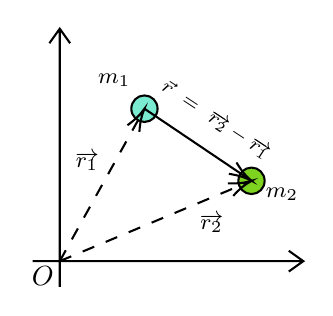
\begin{tikzpicture}[x=0.75pt,y=0.75pt,yscale=-1,xscale=1]
%uncomment if require: \path (0,178); %set diagram left start at 0, and has height of 178

%Shape: Axis 2D [id:dp42543499801858453] 
\draw  (222.72,138.99) -- (353.11,138.99)(235.76,27) -- (235.76,151.44) (346.11,133.99) -- (353.11,138.99) -- (346.11,143.99) (230.76,34) -- (235.76,27) -- (240.76,34)  ;
%Shape: Ellipse [id:dp34665186673267967] 
\draw  [fill={rgb, 255:red, 80; green, 227; blue, 194 }  ,fill opacity=0.76 ] (270.24,65.54) .. controls (270.24,62.01) and (273.08,59.14) .. (276.57,59.14) .. controls (280.06,59.14) and (282.89,62.01) .. (282.89,65.54) .. controls (282.89,69.07) and (280.06,71.93) .. (276.57,71.93) .. controls (273.08,71.93) and (270.24,69.07) .. (270.24,65.54) -- cycle ;
%Shape: Ellipse [id:dp9968570486343863] 
\draw  [fill={rgb, 255:red, 126; green, 211; blue, 33 }  ,fill opacity=1 ] (321.82,100.29) .. controls (321.82,96.76) and (324.65,93.9) .. (328.15,93.9) .. controls (331.64,93.9) and (334.47,96.76) .. (334.47,100.29) .. controls (334.47,103.82) and (331.64,106.68) .. (328.15,106.68) .. controls (324.65,106.68) and (321.82,103.82) .. (321.82,100.29) -- cycle ;
%Straight Lines [id:da8232147057285761] 
\draw  [dash pattern={on 4.5pt off 4.5pt}]  (235.76,138.99) -- (275.6,67.29) ;
\draw [shift={(276.57,65.54)}, rotate = 119.06] [color={rgb, 255:red, 0; green, 0; blue, 0 }  ][line width=0.75]    (10.93,-3.29) .. controls (6.95,-1.4) and (3.31,-0.3) .. (0,0) .. controls (3.31,0.3) and (6.95,1.4) .. (10.93,3.29)   ;
%Straight Lines [id:da9672340288452689] 
\draw  [dash pattern={on 4.5pt off 4.5pt}]  (235.76,138.99) -- (326.3,101.06) ;
\draw [shift={(328.15,100.29)}, rotate = 157.27] [color={rgb, 255:red, 0; green, 0; blue, 0 }  ][line width=0.75]    (10.93,-3.29) .. controls (6.95,-1.4) and (3.31,-0.3) .. (0,0) .. controls (3.31,0.3) and (6.95,1.4) .. (10.93,3.29)   ;
%Straight Lines [id:da6937866085380056] 
\draw    (276.57,65.54) -- (326.49,99.17) ;
\draw [shift={(328.15,100.29)}, rotate = 213.97] [color={rgb, 255:red, 0; green, 0; blue, 0 }  ][line width=0.75]    (10.93,-3.29) .. controls (6.95,-1.4) and (3.31,-0.3) .. (0,0) .. controls (3.31,0.3) and (6.95,1.4) .. (10.93,3.29)   ;

% Text Node
\draw (241.74,85.16) node [anchor=north west][inner sep=0.75pt]  [font=\footnotesize]  {$\overrightarrow{r_{1}}$};
% Text Node
\draw (301.74,114.97) node [anchor=north west][inner sep=0.75pt]  [font=\footnotesize]  {$\overrightarrow{r_{2}}$};
% Text Node
\draw (287.5,48.56) node [anchor=north west][inner sep=0.75pt]  [font=\scriptsize,rotate=-33.42]  {$\vec{r} \ =\ \overrightarrow{r_{2}} -\overrightarrow{r_{1}}$};
% Text Node
\draw (220.81,140.09) node [anchor=north west][inner sep=0.75pt]    {$O$};
% Text Node
\draw (252.77,47.33) node [anchor=north west][inner sep=0.75pt]  [font=\footnotesize]  {$m_{1}{}$};
% Text Node
\draw (333.58,102.38) node [anchor=north west][inner sep=0.75pt]  [font=\footnotesize]  {$m_{2}{}$};


\end{tikzpicture}
